\documentclass[twocolumn]{article}
\usepackage{hyperref}
\usepackage[toc,page]{appendix}
\usepackage{amsmath}
\usepackage{graphicx}
\usepackage{subfloat}
\usepackage{multicol}
\usepackage{gensymb}

\graphicspath{{./figures}}

\title{Thermodynamic Simulation of Rocket Nosecones During Ascent}
\author{Eric Souder}
\date{July 2022}

\begin{document}
\twocolumn[\begin{@twocolumnfalse}
\maketitle
    \begin{abstract}
            Method of modeling the heating of rocket vehicle nosecones, and application of
            the model in simulating the temperature change in UBC Rocket's Whistler-Blackcomb 
            flight to 100 km. The simulation results
            show that the nosecone rapidly heats to 540K and plateaus at this temperature. It is 
            concluded that care must be taken in the design of the vehicle to choose nosecone materials
            that can withstand this heat and to appropriately insulate sensitive electronics 
            in the nosecone to ensure they function over the entire flight.
        \end{abstract}

    \end{@twocolumnfalse}
]
    \section{Introduction}
        During the launch of a sounding rocket into suborbital flight, the 
        exterior of the vehicle experiences heat loading, concentrated
        towards the angled nosecone face of the rocket that directly encounters
        the air stream as it accelerates upward. Insight into the 
        specifics of this heating is critical in the design process to ensure 
        that a rocket vehicle is constructed out of materials that will not fail
        and in a manner that maintains internal temperatures at appropriate levels for 
        components housed inside the nosecone. This knowledge is critical not 
        only to the success of the mission, but also the safety of observers and 
        operators in the vicinity of the spacecraft. For this reason, modeling of the
        nosecone has been investigated by many authors over many years.
        This paper incorporates results and ideas from previous works to present
        a simple model of nosecone heating for a suborbital rocket and a simulation, 
        using this model, of an ascent of UBC Rocket's Whistler-Blackcomb vehicle 
        to roughly 100 kilometers.

    \section{Modeling Nosecone Skin Heating}
        Objects traveling at high speeds are subject to heating and cooling as 
        they travel through the atmosphere. As a rocket vehicle travels at 
        supersonic velocities, there are two significant contributions to 
        the temperature change of the nosecone - the aerodynamic heating from 
        the compression of air as the nosecone pushes through it, and the heat
        lost to the atmosphere through radiation. For the purposes of this 
        analysis, these will be the only sources of thermal energy change
        considered.
        \subsection{Nosecone Aerodynamic Heating}
            \label{sub:aeroeffect}
            As the nosecone travels at supersonic speeds, it forms a shock wave
            as it moves faster than the air can escape. From the frame of reference of the vehicle, 
            This can be considered as air being blown towards a stationary nosecone, at the
            speed the rocket would be traveling. At the very tip of
            the nosecone, the air has zero relative velocity to the vehicle. 
            This is the stagnation point. \cite{nasa:stagtemp}

            At the stagnation point, all the kinetic energy of the air is 
            converted into thermal energy. Because this process happens so
            quickly, it can be modeled as an adiabatic compression of gas.

            \[PV^\gamma = \textrm{constant}\]

            The ideal gas approximation ($V\propto TP^{-1}$) can be applied, so 

            \[P^{1-\gamma}T^\gamma=\textrm{constant}\]

            In our compression, this means 

            \[\frac{T_s}{T_0}=\left(\frac{P_s}{P_0}\right)^\frac{\gamma-1}{\gamma}\]

            With $T_s, P_s$ as the stagnation temperature and pressure and 
            $T_0, P_0$ as the static temperature and pressure. The relation 
            between the static and stagnation pressure of a gas is sourced from 
            a National Advisory Committee for Aeronautics report on compressible 
            flow \cite{naca:compressible}:

            \[\frac{P_s}{P_0} =\left(1+\frac{\gamma-1}{2}M^2\right)^{\frac{\gamma}{\gamma-1}}\]

            Where $M$ is the mach number. This provides an equation for
            stagnation temperature as a function of speed:

            \[\frac{T_s}{T_0}=1+\frac{\gamma-1}{2}M^2\]

            Of course, the entire nose cone will not encounter air at the
            stagnation temperature. Most air will be slowed, but stopped by skin 
            friction with the vehicle, forming a boundary later around the nosecone. 
            Toft models the average temperature of this boundary layer air ($T_B$) based on
            $K$, a temperature recovery factor \cite{Hans:Aero}:

            \[K=\frac{T_B-T_0}{T_s-T_0}\]

            Eber provides a value of $K=0.89$ for cones with vertex
            angles between 20 and 50 degrees \cite{Eber:nazi}.

            We then have an equation for the temperature of the boundary layer:

            \[T_B=KT_s+T_0\left(1-K\right)\]

            Eber also provides an experimentally modeled value for $h$, the heat
            transfer function\footnote{Note that this equation is accurate only 
            for values of $\mu, k, l$, etc. in the US customary system. When determining this value for use in simulations,
            care should be taken to mind unit conversions.} \cite{Eber:nazi}:
            
            \[h=\left(0.0071+0.0154 \sqrt[2]{\beta}\right)\frac{k}{\mu^{0.8}l^{0.2}}\left(\rho_0 u\right)\]

            Based on $k$, the thermal conductivity of air; $\beta$, the vertex 
            angle of the cone; $\rho$, the density of the air; $\mu$, the dynamic
            viscosity of air; $u$ the velocity of the rocket; and $l$, the 
            length of the cone measured along the surface. 

            With all this, we can determine the heat flux into the nosecone skin
            from aerodynamic effects:

            \[
                \dot{Q}_{aero}= h(T_B-T_N)
            \]

            Where $T_N$ is the actual temperature of the nosecone skin.
            

            \begin{figure}
                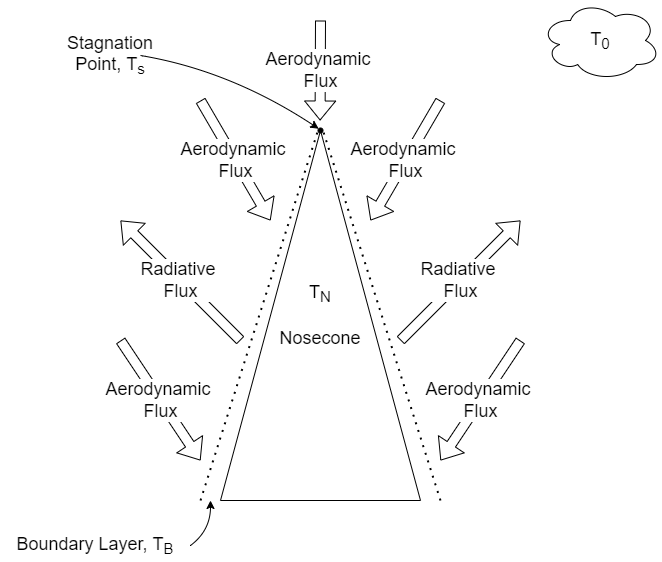
\includegraphics[width=\linewidth]{nosecone.png}
                \caption{Thermal fluxes acting on the nosecone}
                \label{fig:nosecone}
            \end{figure}

        \subsection{Radiative Effects}
            Some amount of heat flux leaves the nosecone as blackbody radiation,
            with heat flux $\dot{Q}_rad=\epsilon\sigma(T_0^4-T_N^4)$, where
            $\epsilon$ is the emissivity of stainless steel and 
            $\sigma$ is the Stefan-Boltzmann constant.

            This situation as well as the effects of section \ref{sub:aeroeffect}
            above is generalized in figure \ref{fig:nosecone}, showing
            the fluxes into and out of the nosecone as well as the locations of 
            the various temperatures used in the calculation. Note that the 
            direction of the flux arrows is generalized, and they may point in 
            opposite directions at different points during the flight.

            %talk about absorption of solar radiation?%

        \subsection{Flight Profile}
            In order to model the thermal behavior of the nosecone, we must
            provide a number of inputs to our aerodynamic heating simulation 
            functions based on altitude and velocity. These inputs are provided 
            by UBC Rocket's proprietary Feynman vehicle design program.
            
            Although Feynman was originally intended for optimizing the design
            of rocket vehicle components, such as fins, engines, or nosecones 
            for maximum altitude without regard for thermal effects, its outputs
            are helpful in the analysis of the nosecones thermal properties. 

            Feynman provides data for Mach number and altitude at 10
            millisecond intervals for the first approximately 160 seconds of
            flight, corresponding to a peak altitude of almost 100 kilometers
            and a maximum speed of more than mach 4. 
            For this reason, we can use the output data of the Feynman
            simulation as a reasonable input flight profile for our thermal
            analysis.

            \begin{subfigures}
                \begin{figure}[h]
                    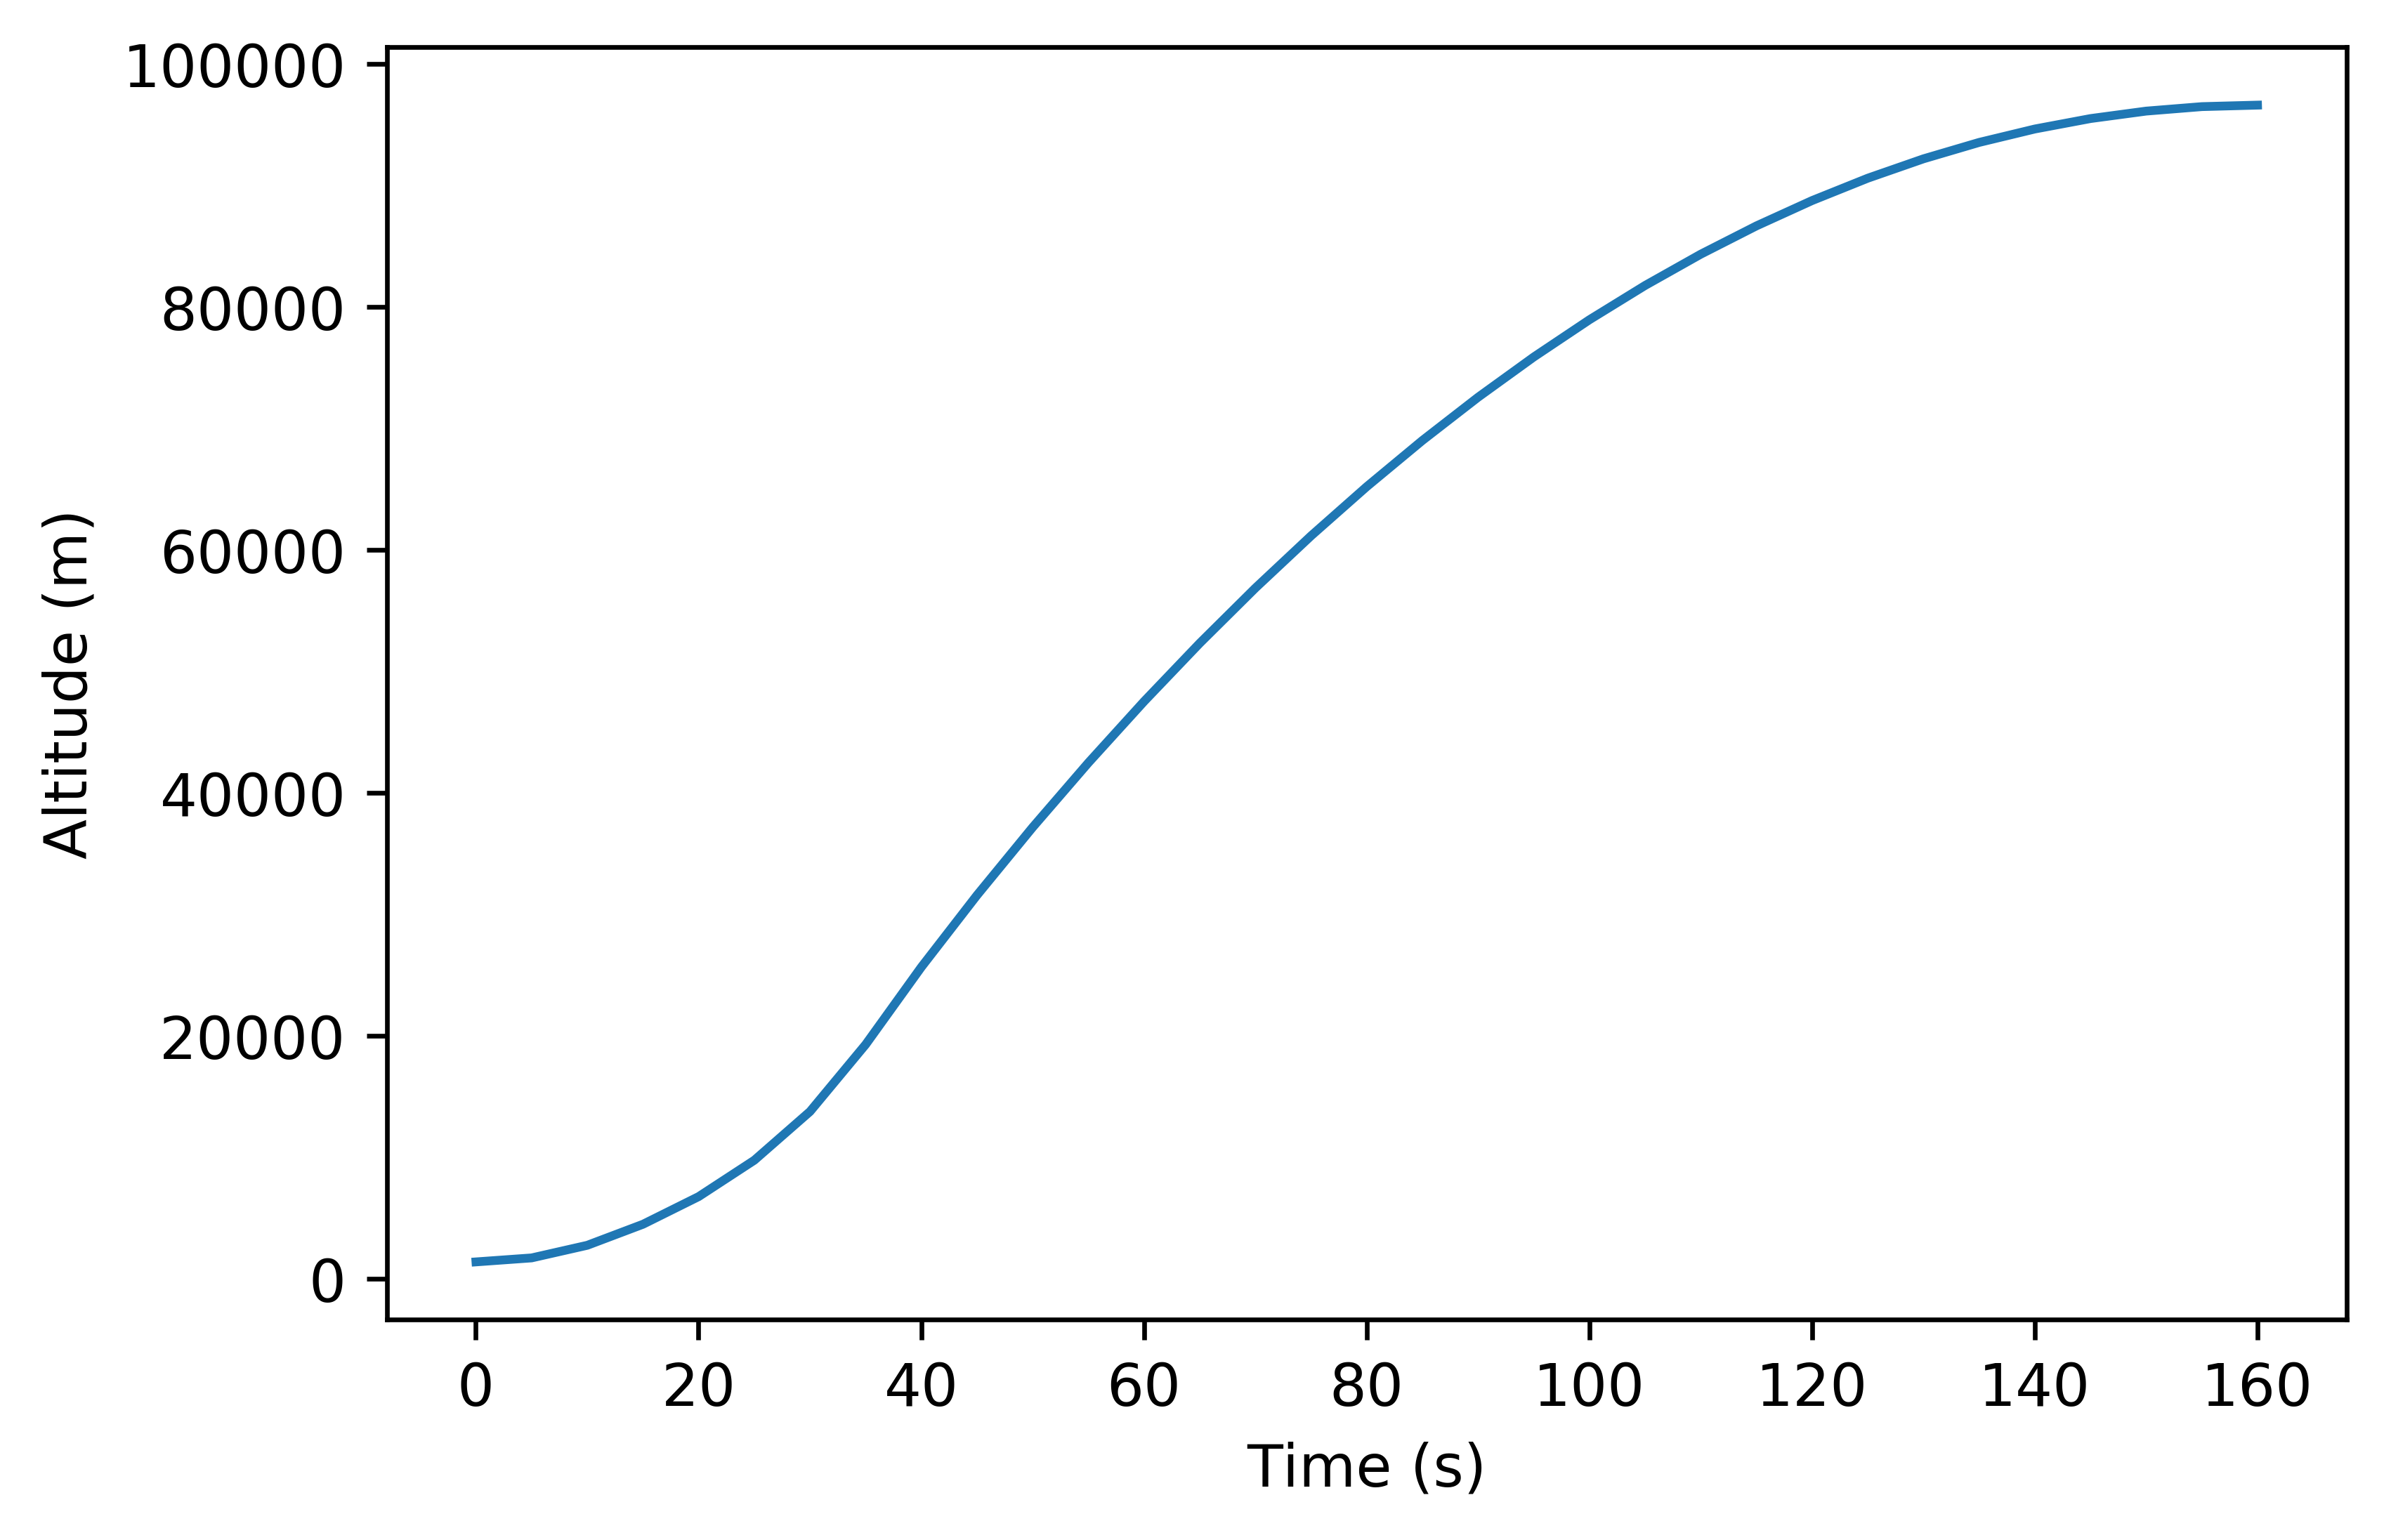
\includegraphics[width=\linewidth]{altitude.png}
                    \caption{Altitude over Time of simulated vehicle trajectory}
                    \label{fig:alt}
                \end{figure}
                \begin{figure}[h]
                    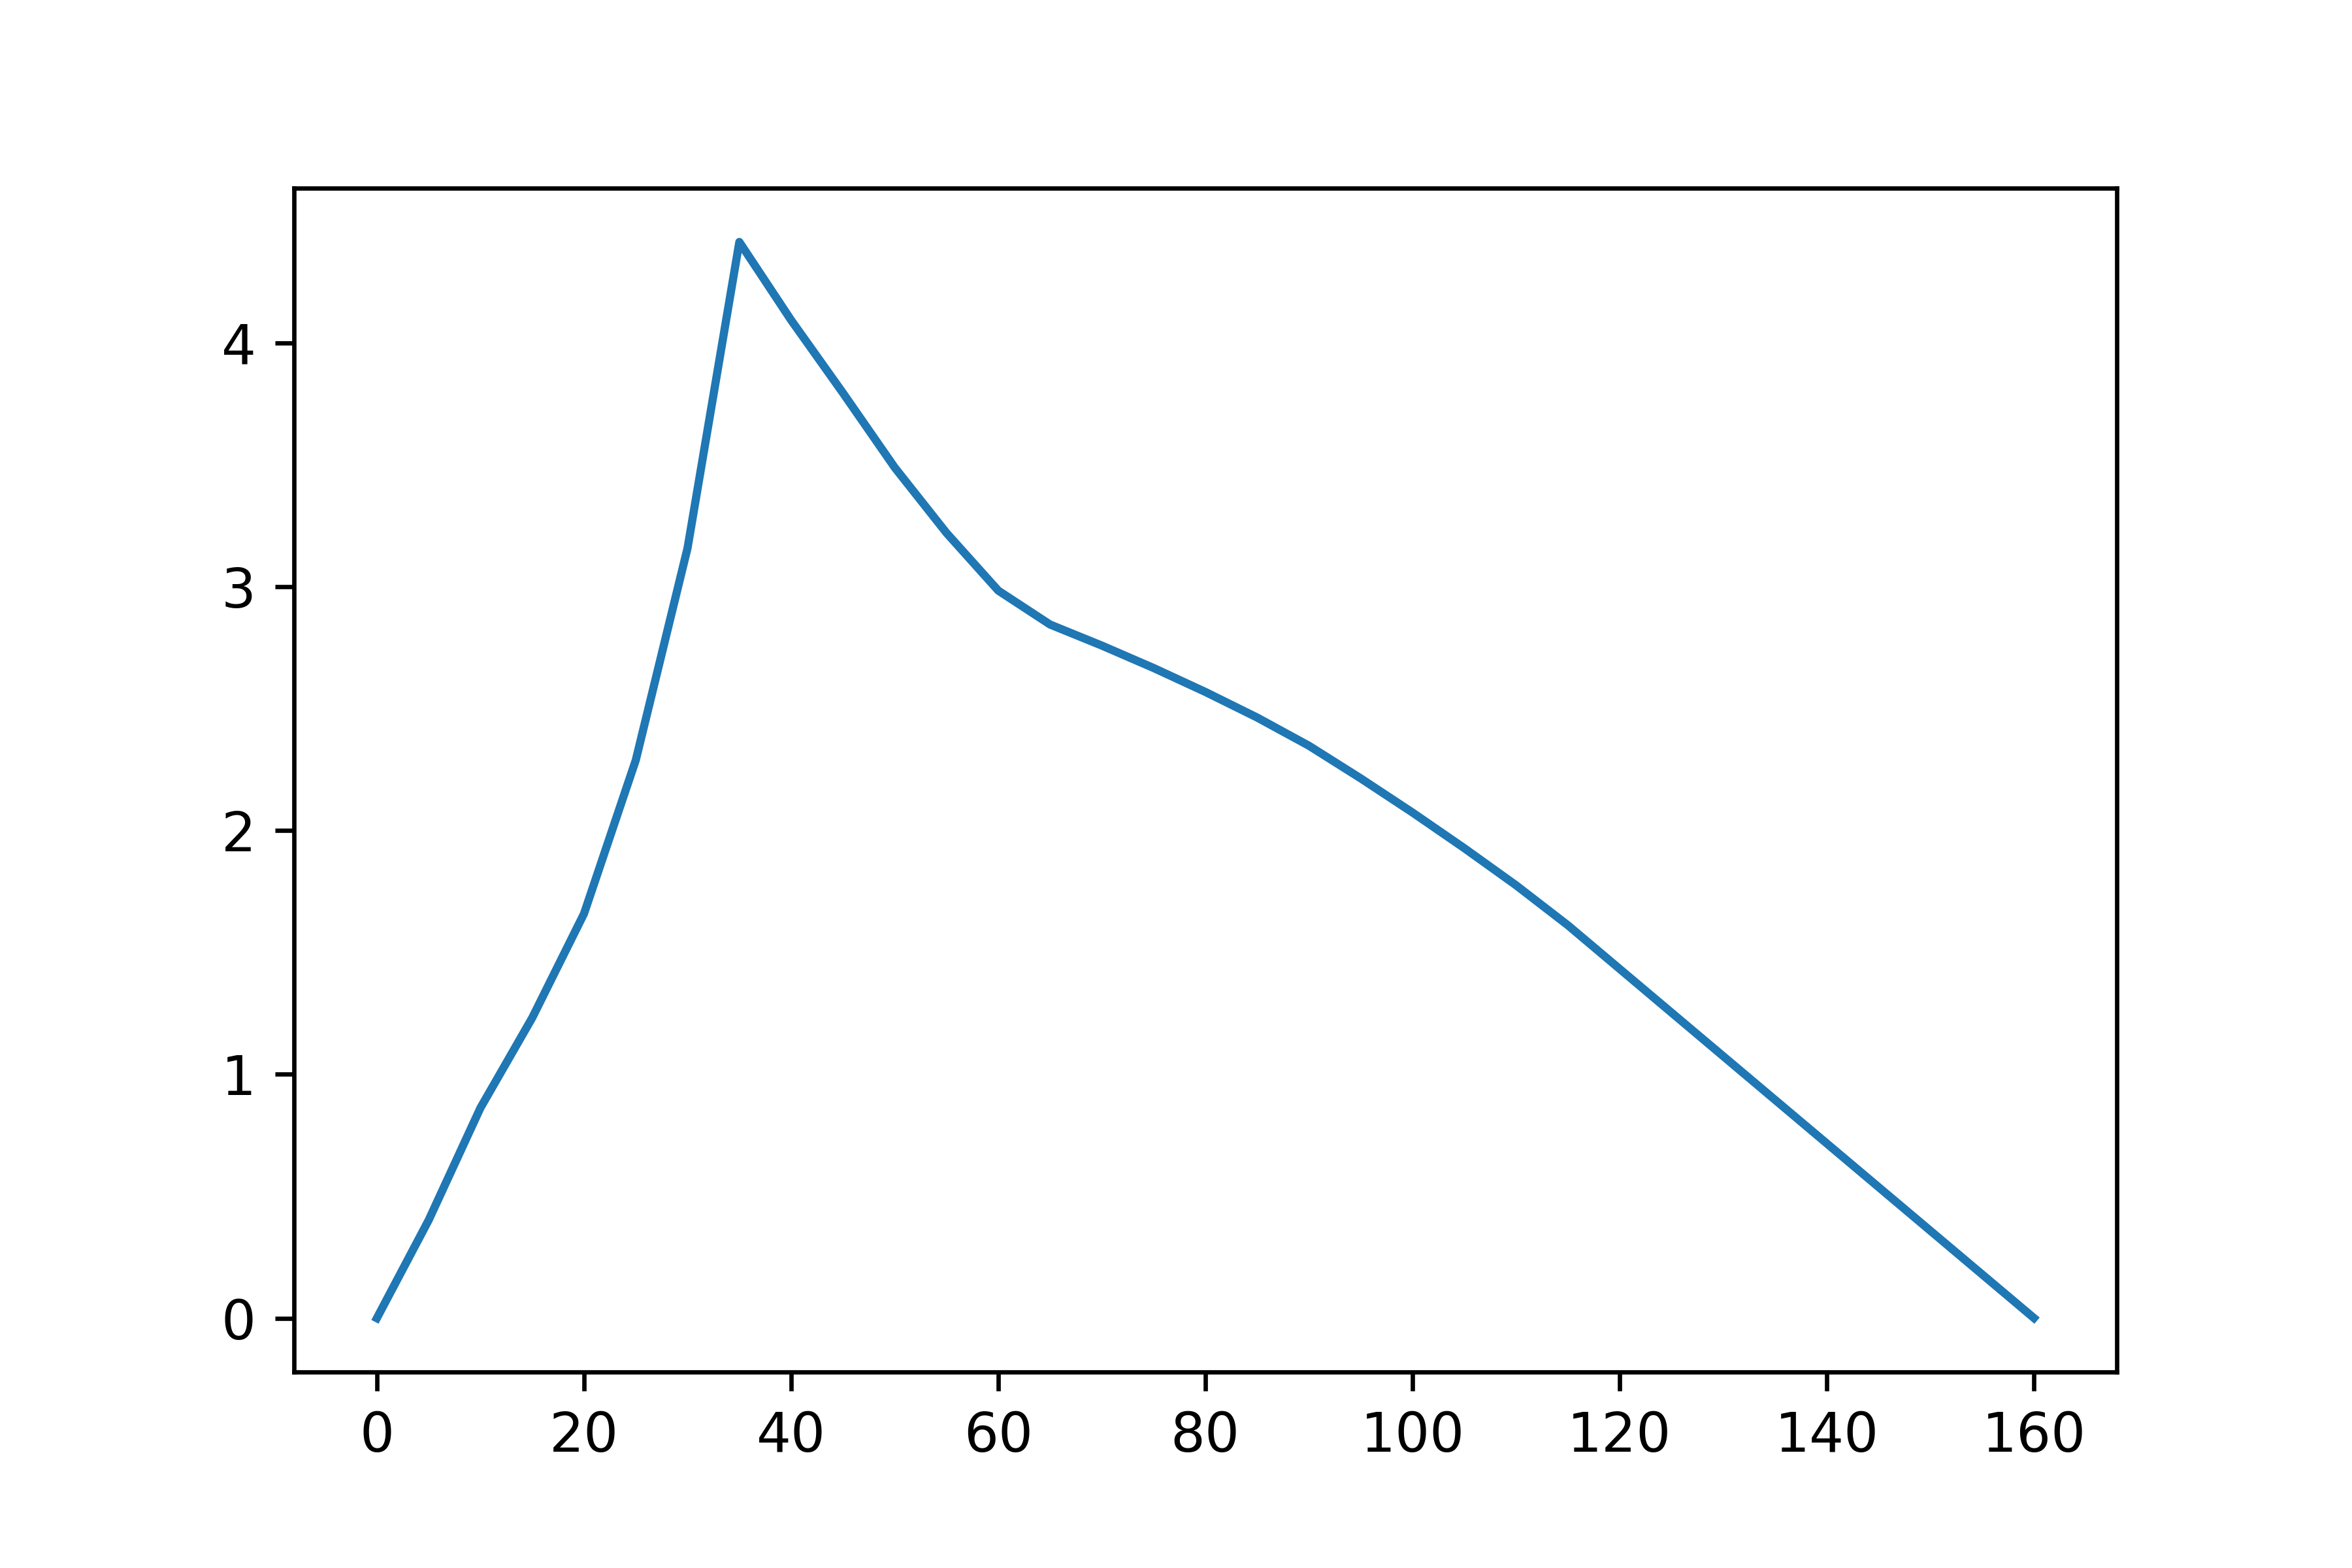
\includegraphics[width=\linewidth]{machs.png}
                    \caption{Mach number over time of simulated vehicle trajectory}
                    \label{fig:mach}
                \end{figure}
            \end{subfigures}

            Additionally, empirically-derived curves
            for $\rho_0$ and  $T_0$ in 
            terms of altitude and of $\mu$ and $k$ in terms of $T_0$ are 
            provided in appendix \ref{appendix:a}. These provide a full picture
            of the conditions around the nosecone over all stages of the flight.
        \subsection{Heat Flux Balance}
            Expanding on the first law of thermodynamics, our simulation must 
            respect the conservation of energy. Thus, the nosecone situation 
            through flight can be modeled by an energy balance:

            \[\textrm{Heat Flux In} = \textrm{Heat Flux out}\]

            This can be modeled by the heat equation:

            \[G dT_N = dt(\dot{Q}_{aero}-\dot{Q}_{rad})\]

            or 

            \begin{equation}
                \label{dTN}
                dT_N = \frac{dt(\dot{Q}_{aero}-\dot{Q}_{rad})}{G}
            \end{equation}

            With a factor $G$, the 'skin heating capacity' \cite{naca:skintemp}
            determined by the specific heat of the nosecone skin $c$, it's 
            thickness $\tau$, and it's density $\rho$.

            \[G=c\tau\rho\]

        \subsection{Simulation Method}

            Considering a small but finite change in time $\Delta t$ (in our 
            simulation case, $10ms$, from Feynman as above), we can
            numerically solve for the change $\Delta T_N$ in the nosecone
            temperature based on equation \ref{dTN} above. 

            This solution is determined by means of a python simulation which
            iterates over each timestep and calculates the change in $T_N$
            for that time. Using the atmospheric models from appendix 
            \ref{appendix:a} and the constant values from appendix 
            \ref{appendix:b}, a representative model of the at-rest (i.e. far
            away from the vehicle's path of flight) is created. Then, using the 
            Feynman-derived data for Mach number and altitude, and the derived
            equations from the above sections, values are determined for $u,
            \mu, k, h, T_s, T_B, \dot{Q}_{aero}$ and $\dot{Q}_{rad}$, which are
            then used to solve for $\Delta T_N$ for the timestep, which then
            modifies $T_N$ for use in the simulation of the next timestep.

    \section{Discussion of Results}

        \subsection{General Discussion}
            Based on the above simulation, the temperature of the nosecone can
            be determined as a function of time as seen in figure 
            \ref{fig:temptime} below. The peak temperature of 540 K occurs
            about 65 seconds into the flight. It is interesting to note that 
            after the rapid rise in temperature, the decline after the peak is 
            significantly shallower, nearly plateauing. 
            
            \begin{figure}[h]
                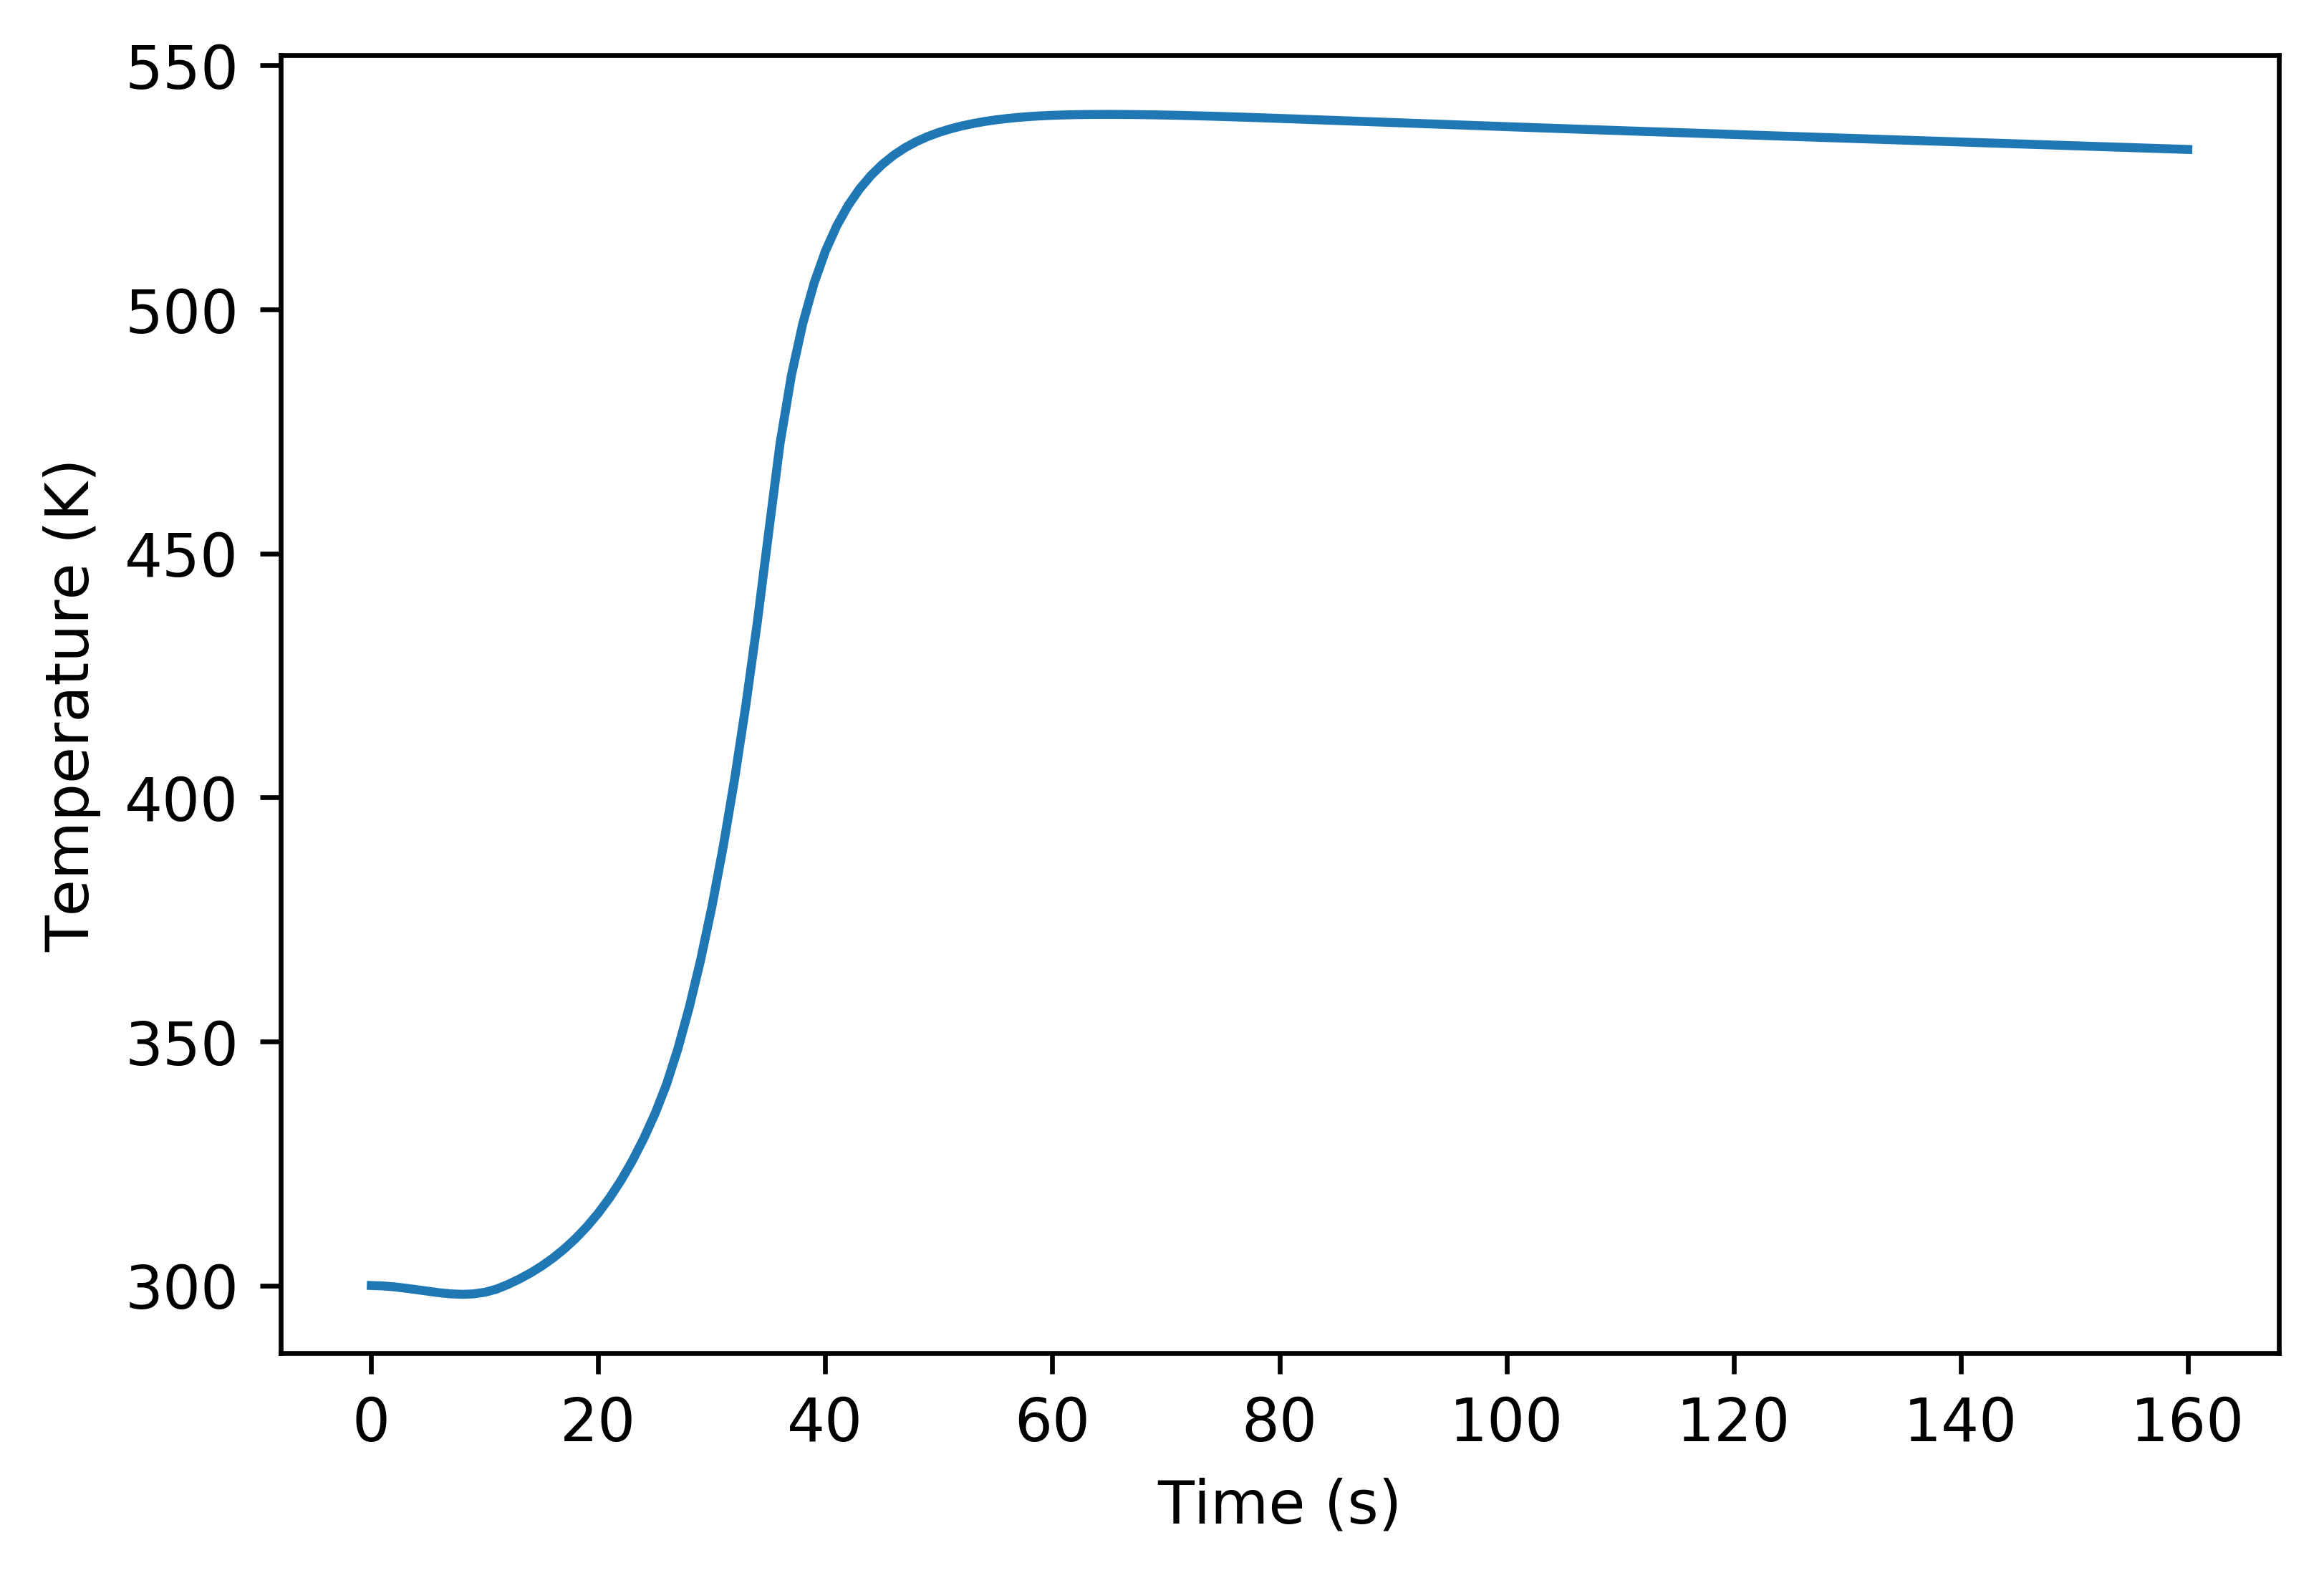
\includegraphics[width=\linewidth]{tempprofile.png}
                \caption{Temperature of nosecone skin over time}
                \label{fig:temptime}
            \end{figure}
            \begin{subfigures}
                \label{fig:flux}
                \begin{figure}[h]
                    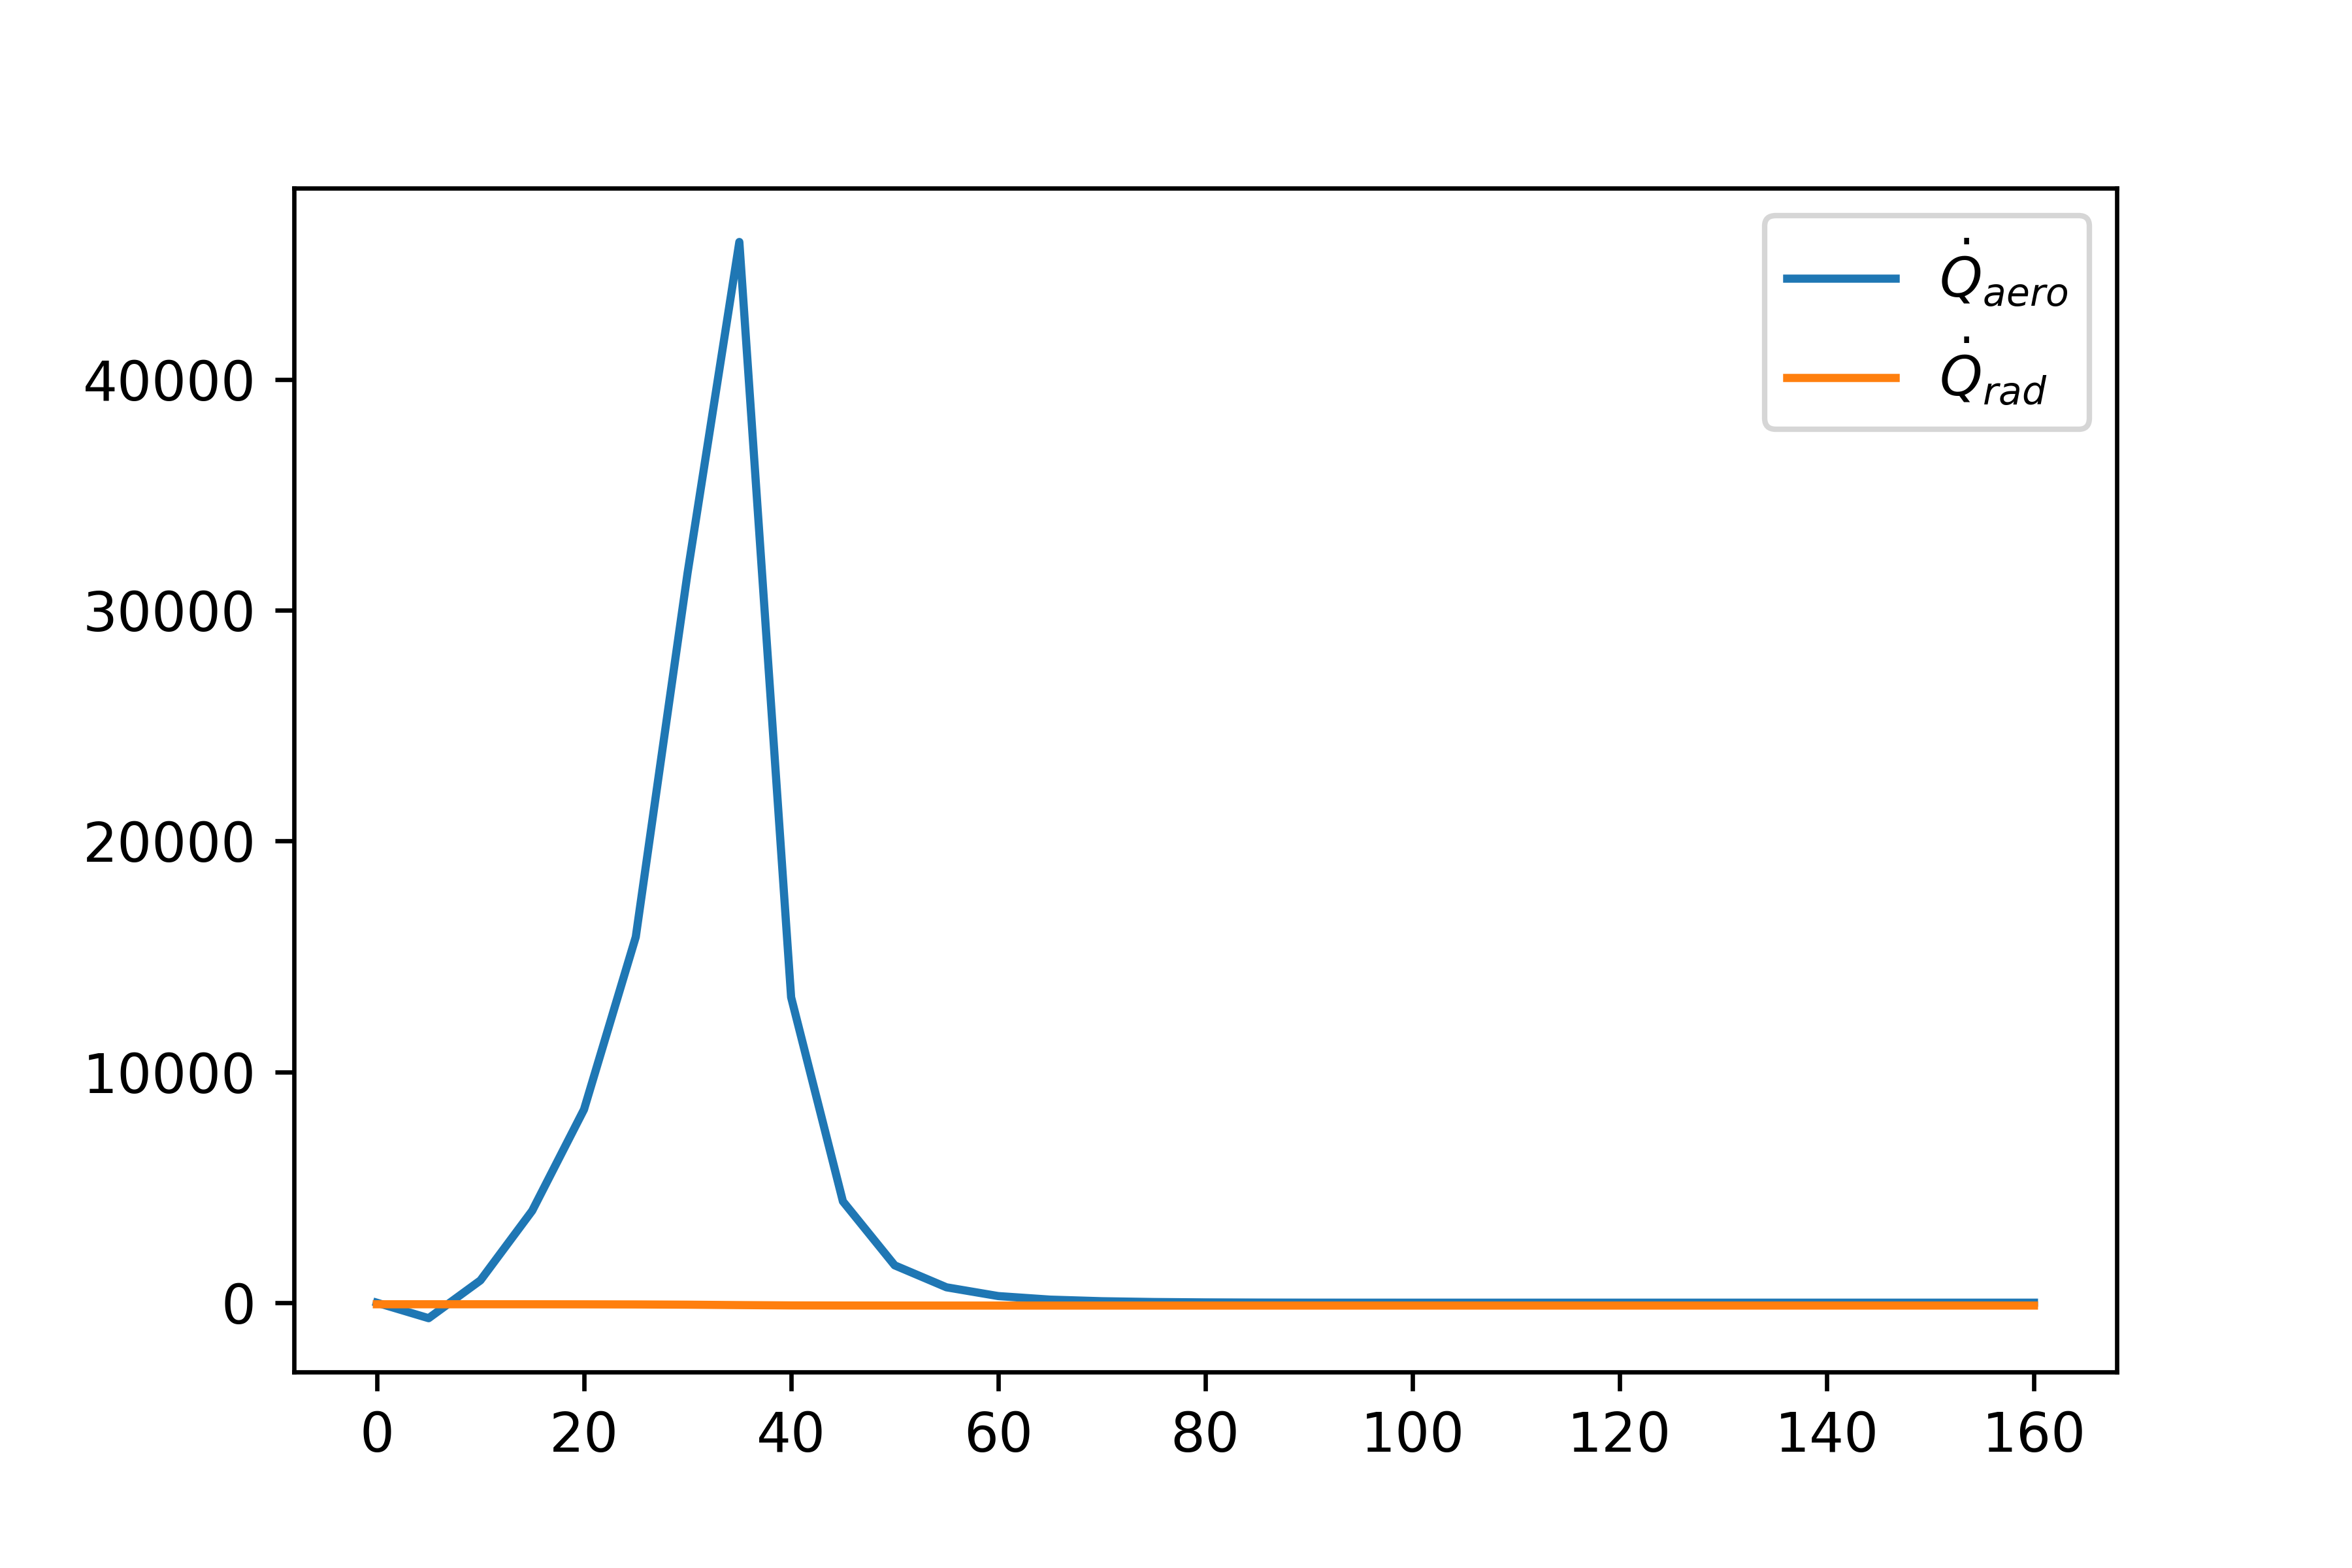
\includegraphics[width=\linewidth]{flux.png}
                    \caption{$\dot{Q}_{aero}$ and $\dot{Q}_{rad}$ fluxes over time}
                    \label{fig:fluxboth}
                \end{figure}
                \begin{figure}
                    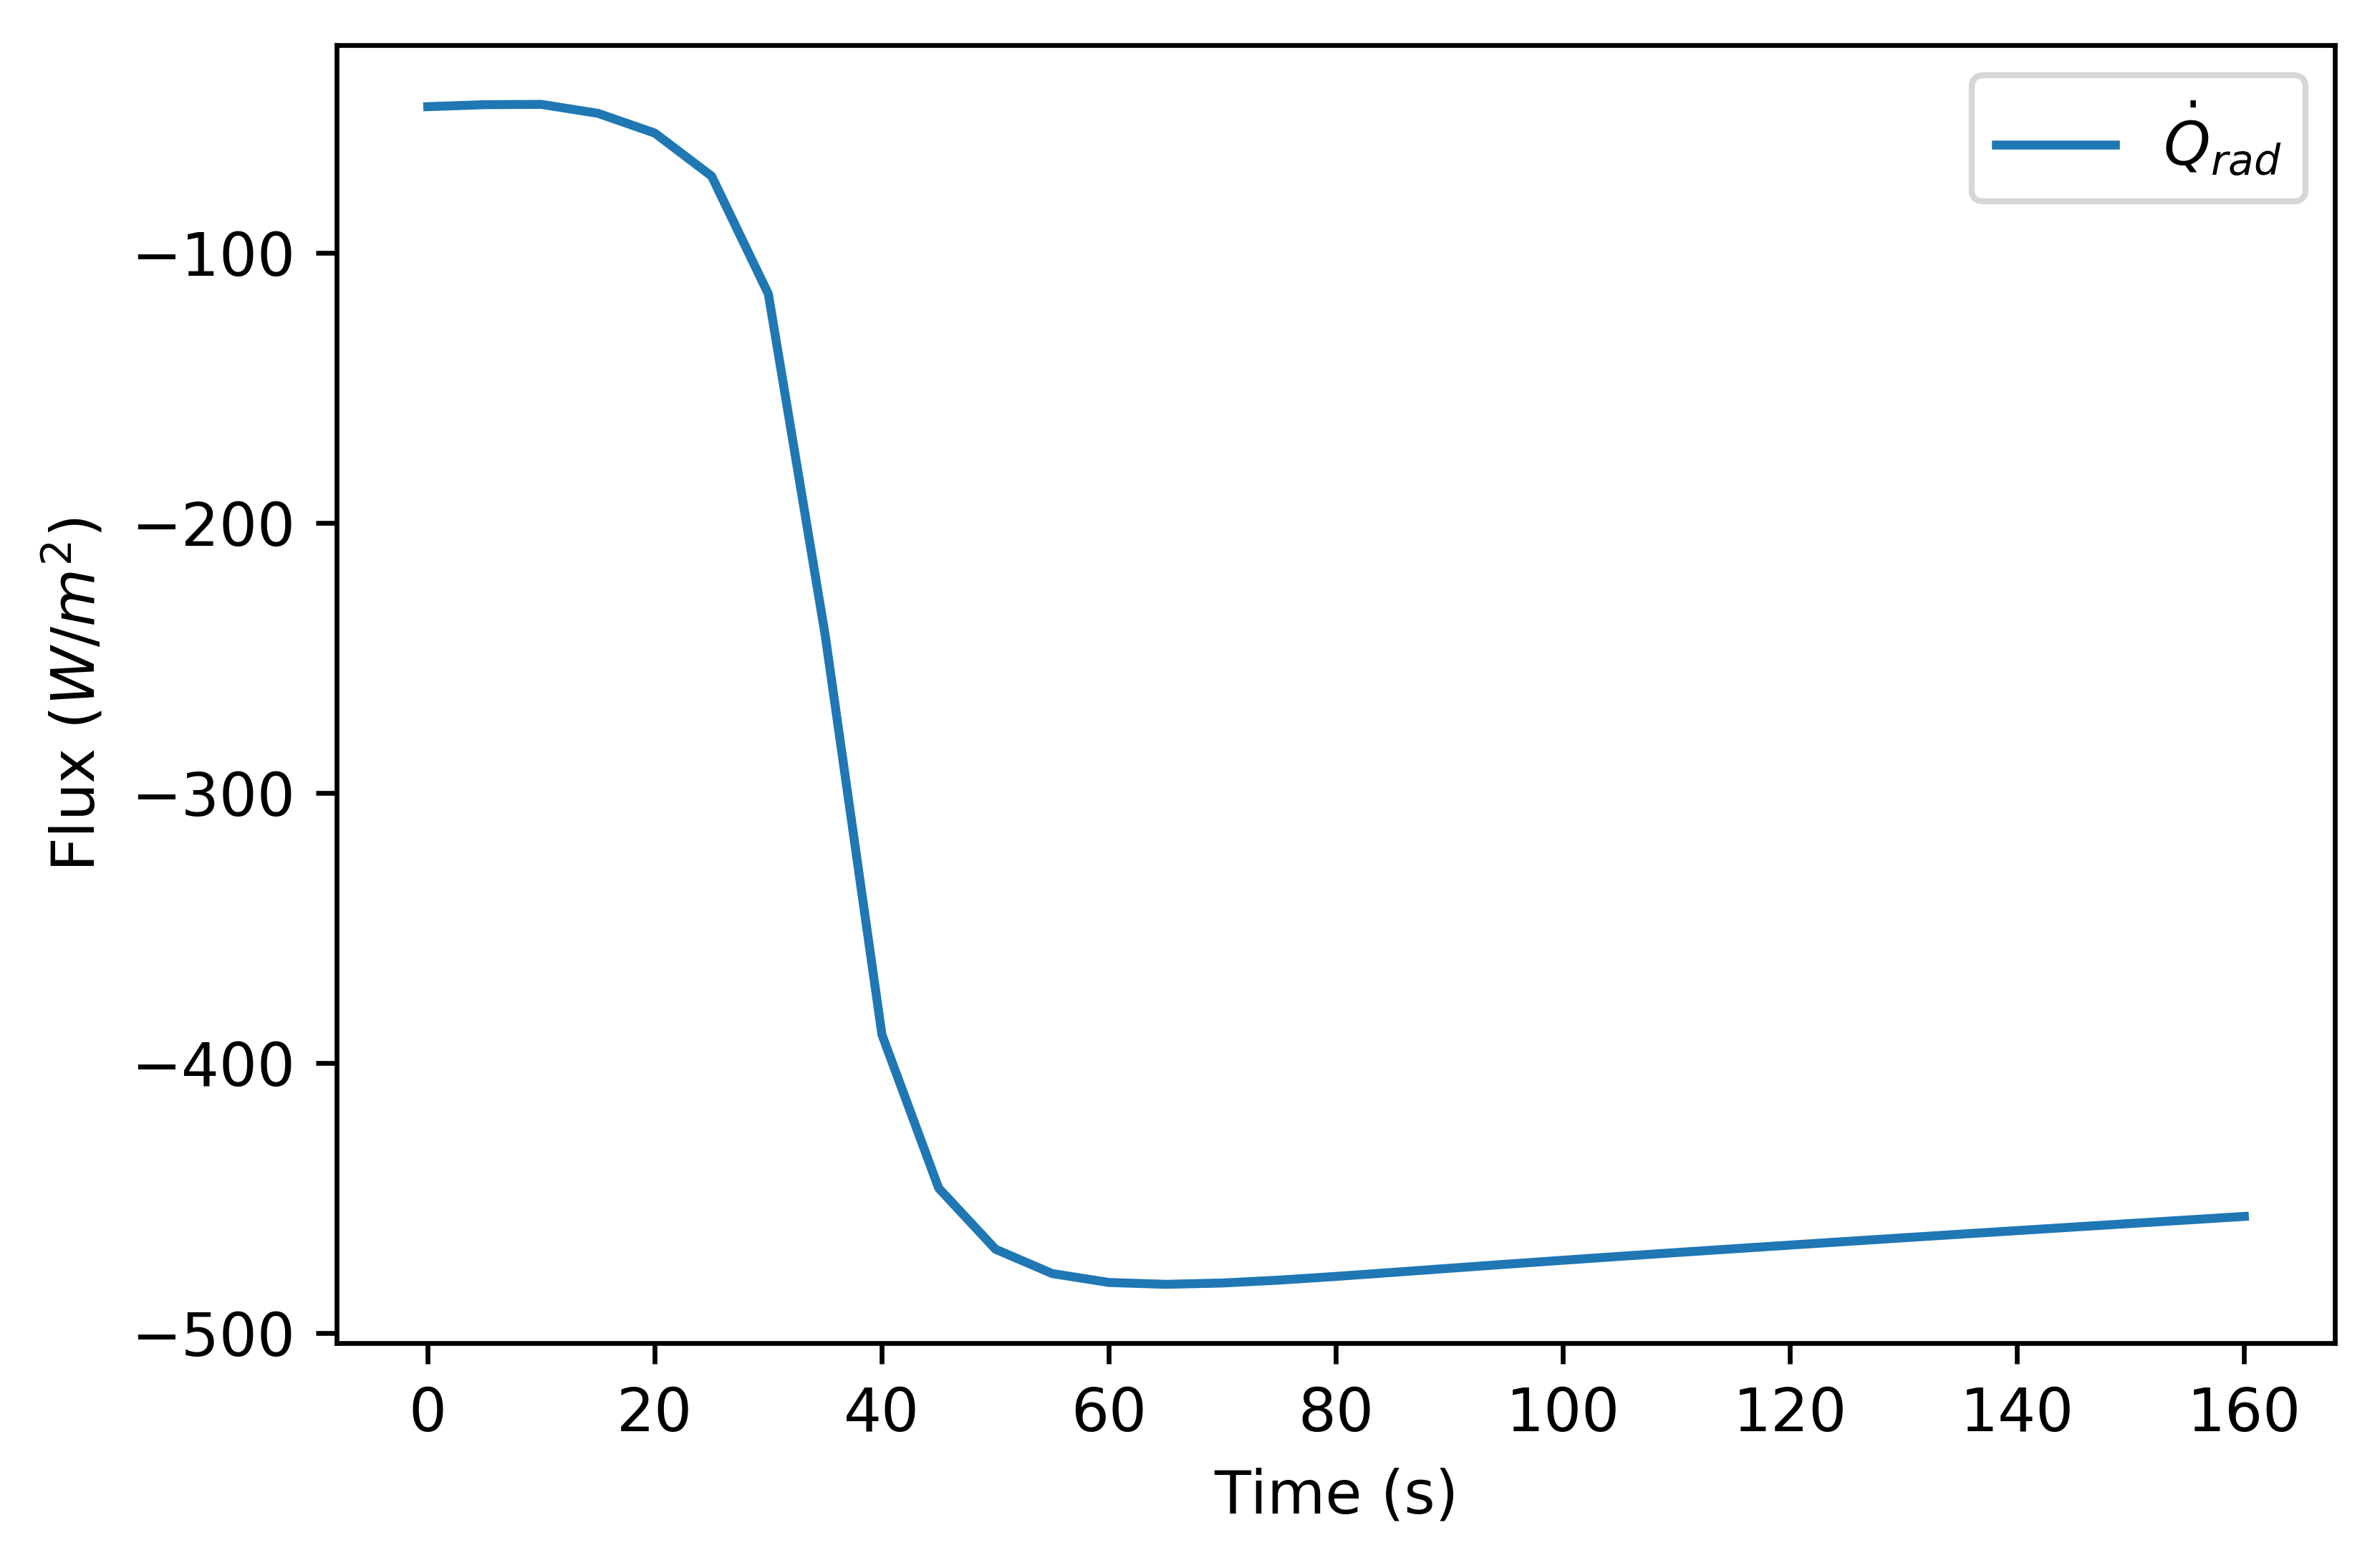
\includegraphics[width=\linewidth]{fluxrad.png}
                    \caption{Detail of $\dot{Q}_{rad}$ flux over time}
                    \label{fig:fluxrad}
                \end{figure}
                
            \end{subfigures}

            This is reasonable considering figure \ref{fig:flux}: the vast majority of the 
            total heat flux at the skin of the rocket is due to aerodynamic
            effects, with the peak of the aerodynamic flux occurring generally at 
            the same time as the peak mach number. This would seem to be a
            reasonable result. Considering the fixed-vehicle frame of reference,
            as air particles encounter the tip of the nosecone at higher speeds, 
            they will have more kinetic energy, all of which will be transferred 
            to the nosecone, increasing the kinetic energy of its constituent 
            particles and so increasing its temperature more than at slower
            velocities. Since we expect the heating of the nosecone to be 
            positively related to the stagnation temperature, we can expect
            higher aerodynamic fluxes at higher speeds. 

            The radiative effects, while not zero, are significantly smaller
            than the aerodynamic effects since the nosecone, while experiencing 
            a large aerodynamic flux, is not heated by a huge degree and so
            does not reach high enough temperatures to have the blackbody 
            radiation play a large role in the total flux.
            Additionally, radiative effects are minimized by the low emissivity 
            of the aluminum nosecone - about 0.1 - as it is quite far from a 
            perfect blackbody. Further, the relatively low contribution of the 
            radiative component to the overall simulation output validates 
            our use of a constant $\epsilon$ in calculating emissivity over the 
            entire flight, even though $\epsilon$ does vary with temperature. 

            Through Wien's displacement law, $\lambda_{\textrm{peak}}= \frac{b}{T_N}$, 
            we can predict the peak wavelength of the nosecone's emitted 
            radiation, as shown in figure \ref{fig:lambda}.

            \begin{figure}[h]
                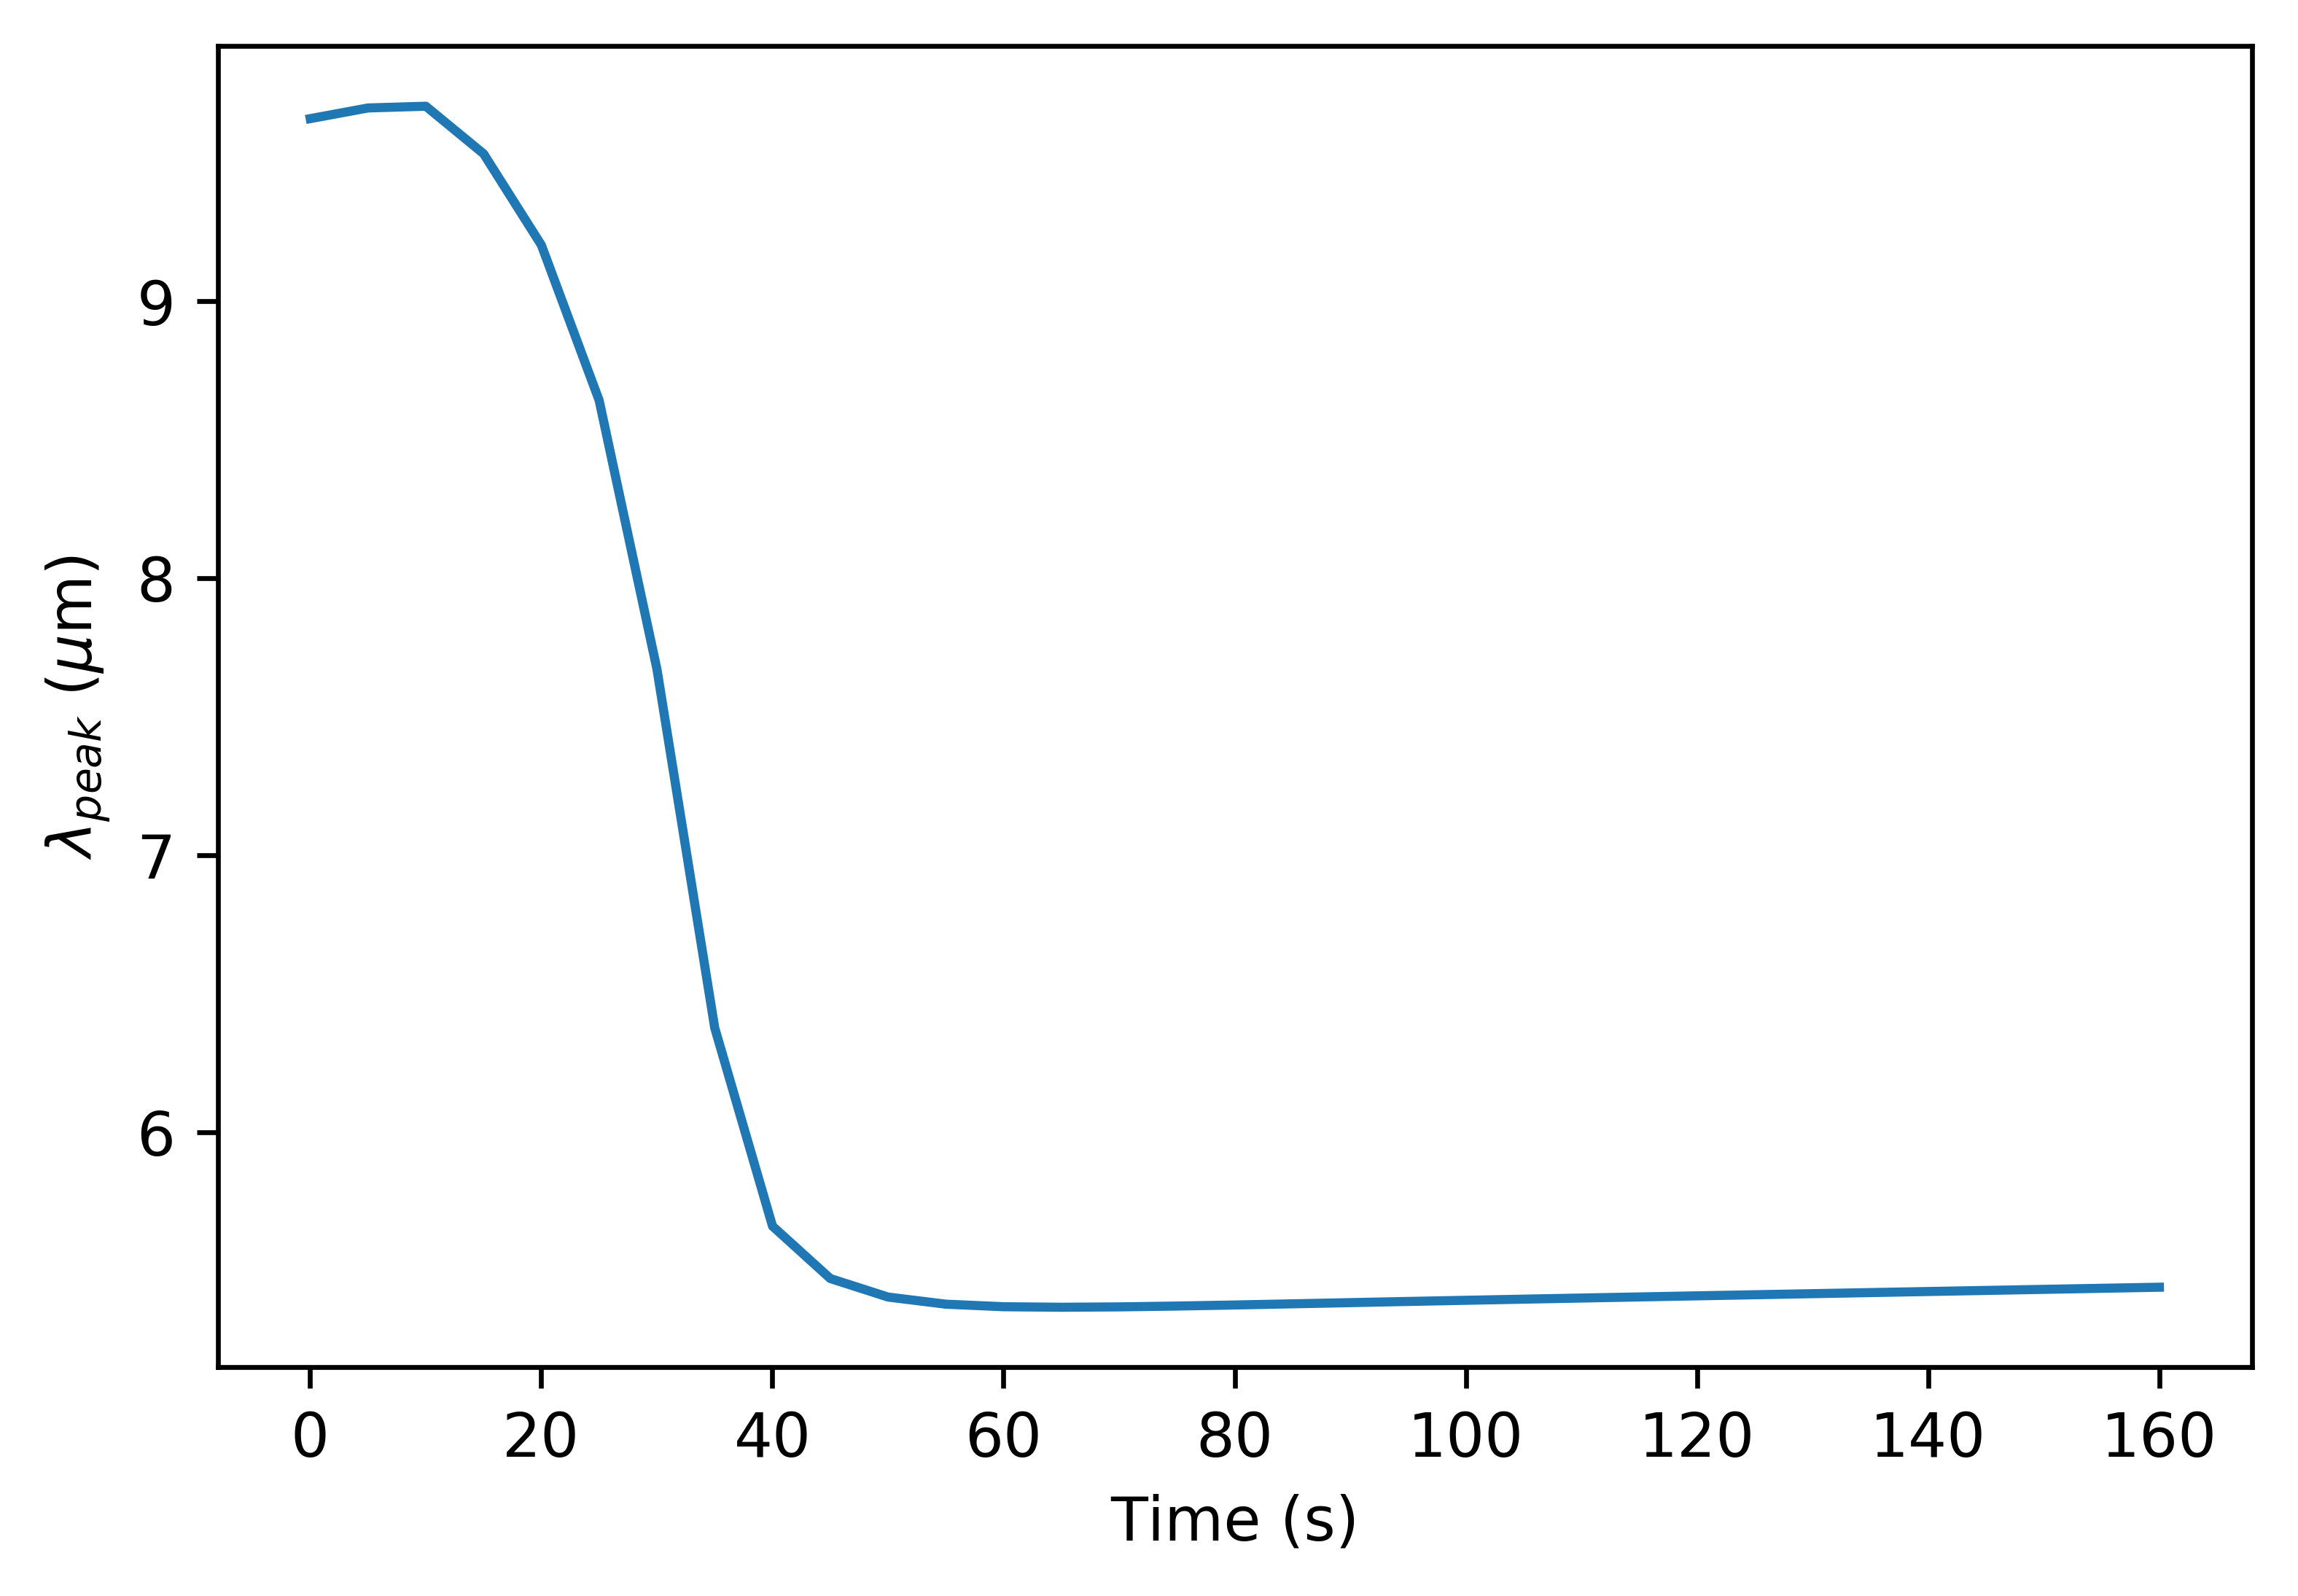
\includegraphics[width=\linewidth]{wavelength.png}
                \caption{Peak wavelength $\lambda_\textrm{peak}$ emitted by the
                nosecone over time}
                \label{fig:lambda}
            \end{figure}

            Since this curve falls strictly within the infrared range, 780 nm to
            1 mm, there will be no visible indication of the temperature of the 
            nosecone.

            We can also predict the temperature of air at the stagnation point
            and boundary layer, seen in figure \ref{fig:boundstagtemps}.
            \begin{figure}[h]
                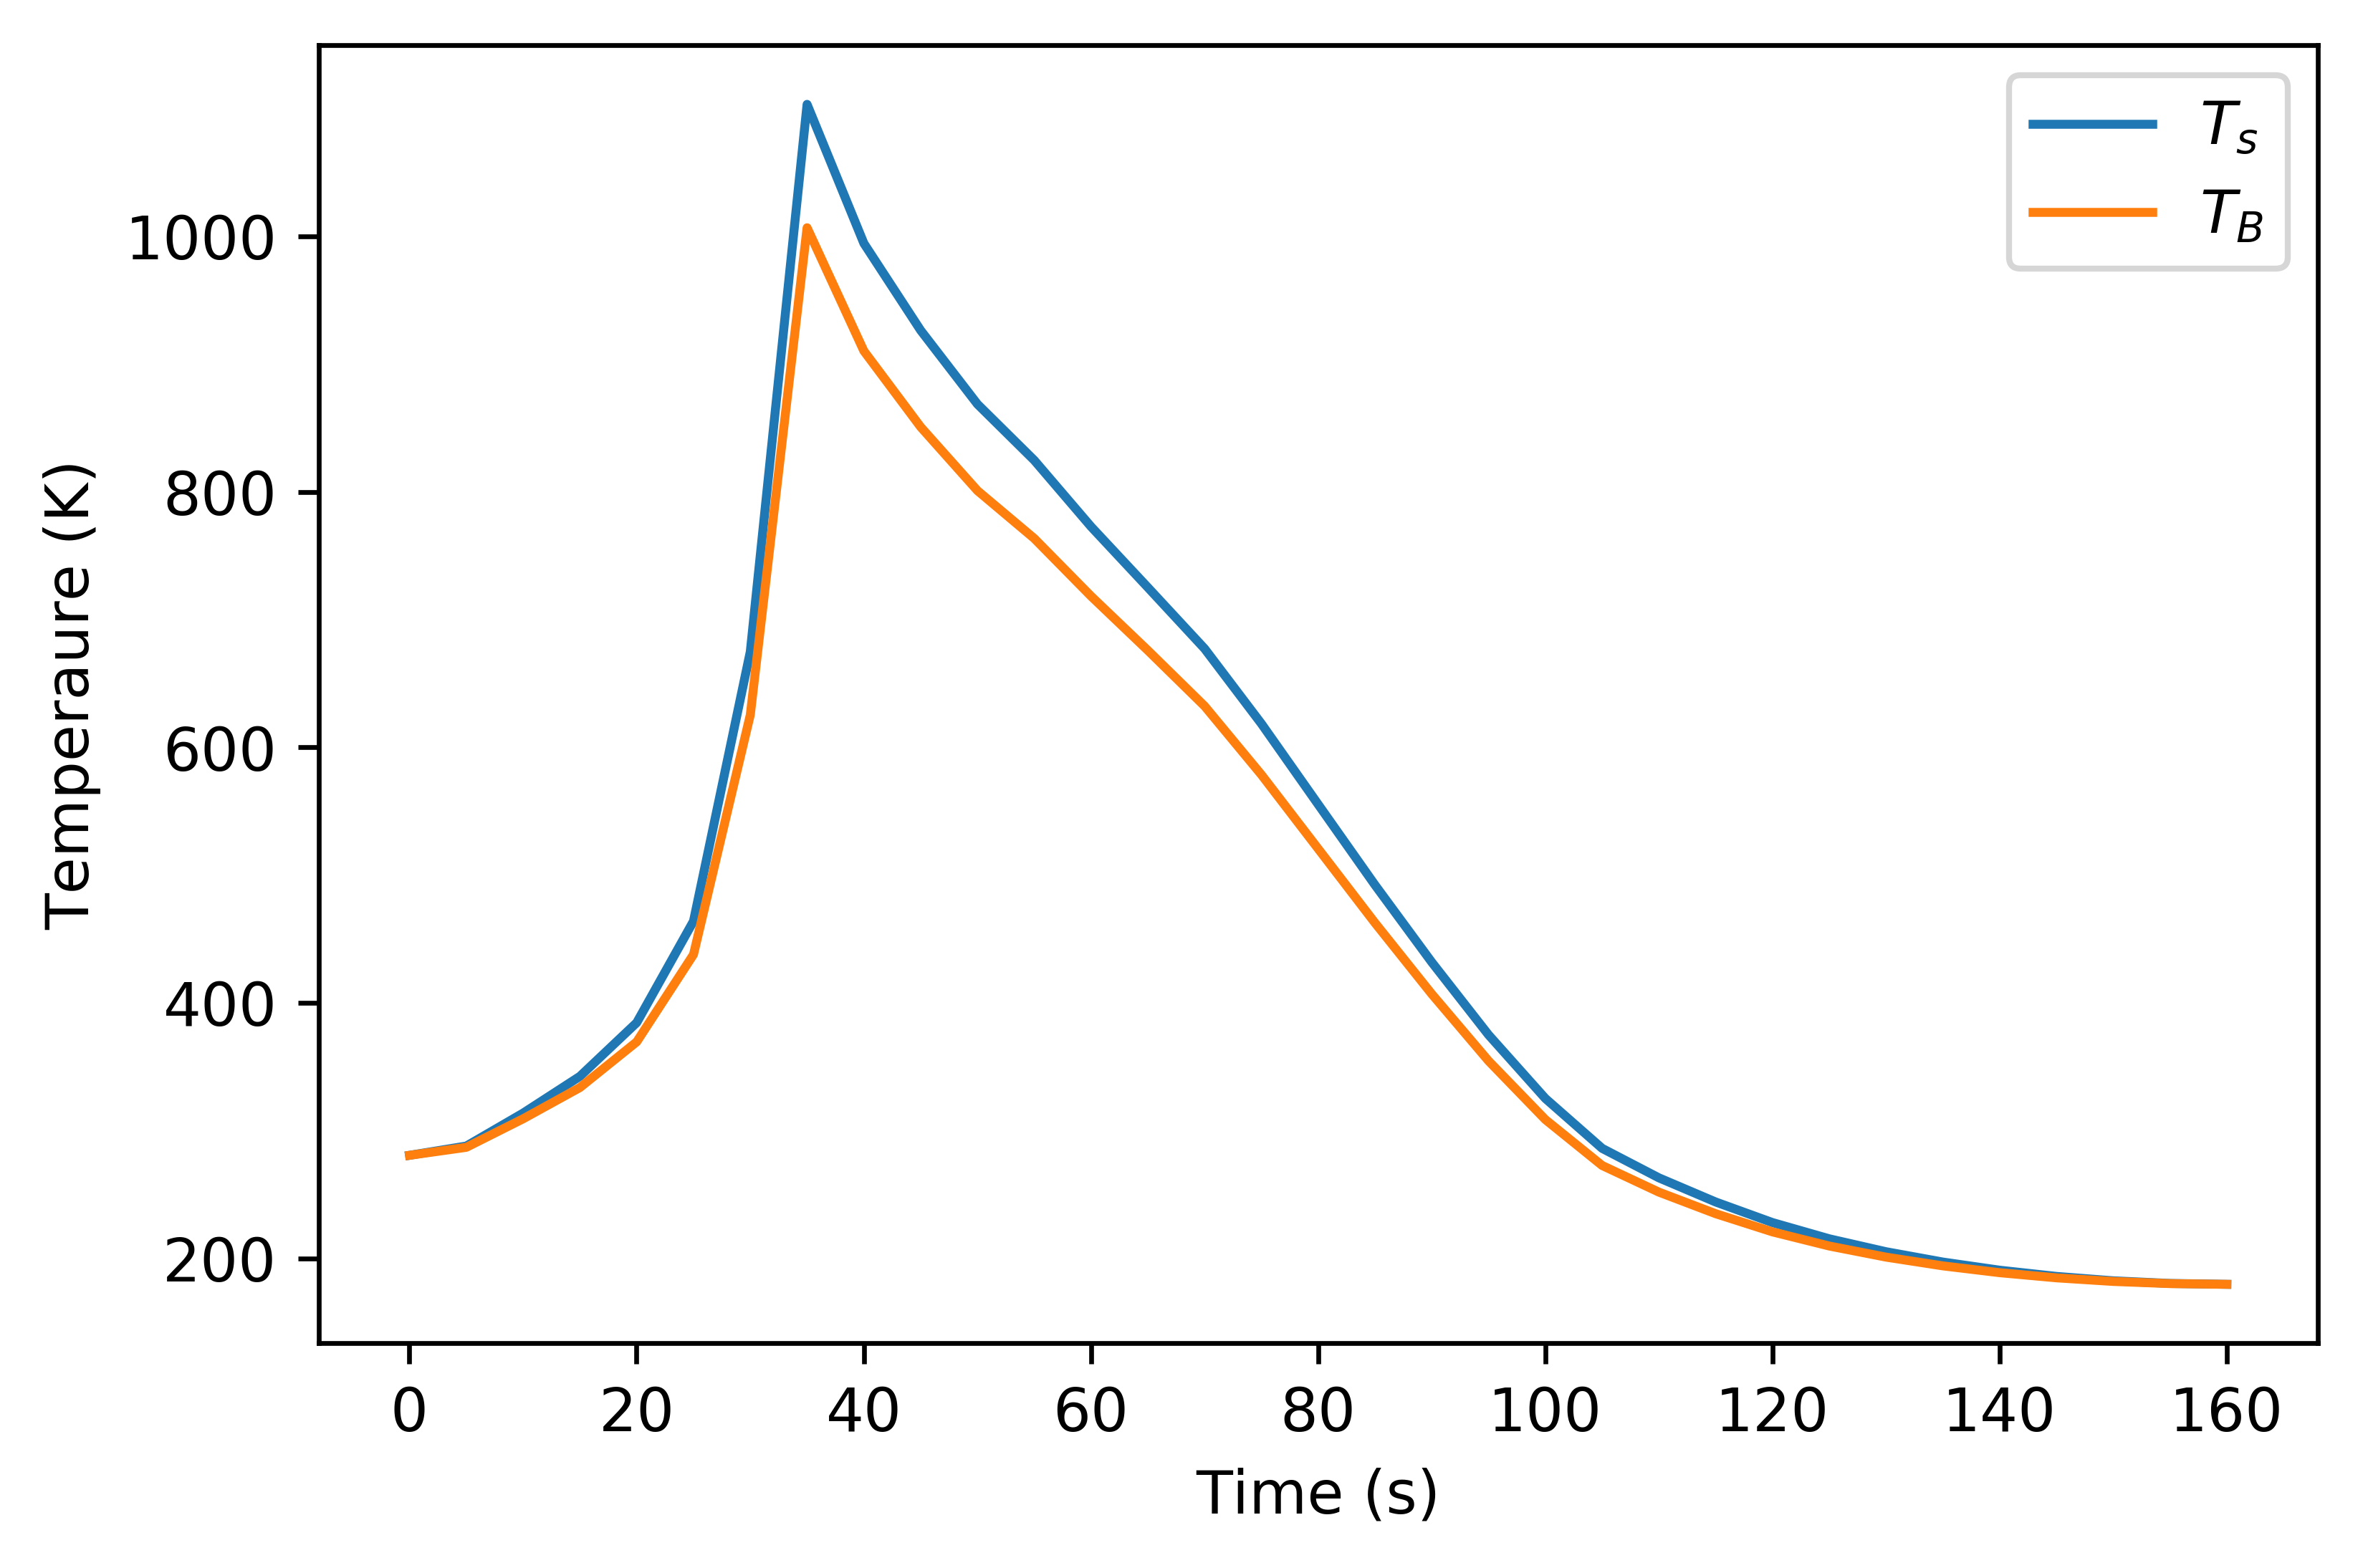
\includegraphics[width=\linewidth]{stagboundtemps.png}
                \caption{Stagnation point and boundary layer temperatures 
                over time}
                \label{fig:boundstagtemps}
            \end{figure}
            
            Although the peak stagnation temperature and boundary layer temperatures
            are quite high, both over 1000K (1139K and 1039K, respectively),
            we do not observe these temperatures in the nosecone skin. 
            Partially, this can be understood from the observation that the 
            peak temperatures occur only briefly, shooting up rapidly and 
            cooling to lower temperatures relatively fast. As well, the aluminum
            has a skin-heating capacity $G$ greater than one, so the change 
            in its temperature is moderated by $G$ in addition to the amount 
            of flux it receives.  
            
            \subsection{Implications for Avionics Hardware Housed in Nosecone}
            Onboard the Whistler-Blackcomb rocket, many of the avionics components
            are housed within the nosecone, including the main flight computer, which
            is responsible for directing most of the primary guidance, navigation, safety, 
            and recovery functions of the avionics system during the flight. For 
            this reason, it is necessary that it functions throughout the entire
            flight. The NXP MK66FX microcontroller chip used in the main flight 
            computer has a maximum ambient temperature rating of 105 degrees Celsius 
            \cite{NXP:K66}, or 378.15K. As this is below the peak temperature
            of the nosecone skin, some care and analysis will be necessary in 
            determining the placement of the flight computer so that it does not 
            reach the same temperature as the nosecone.

            Assuming that the heat capacity of the flight computer is insignificant 
            compared to that of the nosecone - a reasonable assumption since the 
            mass of the flight computer is minimal 
            ($\frac{m_{\textrm{computer}}}{m_\textrm{nosecone}}\approx 0$) - then 
            we know it would be unwise to mount the flight computer directly to
            the interior skin of the nosecone. Considerations will have to be
            made in the placement of avionics, such as thermally insulating it from 
            the metal of the nosecone in order to ensure it continues to function over the duration of 
            the flight. 
            
            If this were a steady state solution, the computer would 
            eventually equilibrate to the temperature of the nosecone and fail.
            However, this plateau is not permanent - it will only last as long as 
            the vehicle remains above an altitude where the $h$, the heat transfer 
            coefficient is low and at speeds where atmospheric heating is a factor.
            At slow speeds with denser atmosphere, the aerodynamic flux reverses
            direction and moves energy from the high-temperature nosecone into the 
            lower-temperature air. 
            
            Since we know the flight plan includes a long,
            slow descent from the upper atmosphere under ballutes and parachutes, 
            design considerations do not need to be made to isolate the flight computer
            from the nosecone plateau temperature for an arbitrarily long amount of time, 
            but for a finite time (measured in minutes) until the nosecone can 
            be sufficiently cooled during reentry. However, more Feynman simulations
            at longer time intervals are needed to accurately determine this time. 

    \section{Conclusions}
        The thermodynamic behavior of the UBC Rocket Whistler-Blackcomb vehicle's 
        nosecone during launch was determined by means of a numerical simulation.
        The analysis showed that under a predicted flight
        profile reaching about 100 km in height at a maximum mach number of about
        4, the average temperature of the nosecone skin reaches 540 K, an increase
        of 240 C from its initial temperature before launch. Based on this analysis,
        The analysis shows also that the heat increases rapidly during launch and then
        plateaus, presenting a concern for temperature-sensitive components housed 
        inside the nosecone.

        Additionally, this paper provides a generalized system of equations that
        can be used to solve by simulation the nosecone temperatures of a nosecone
        under various flight profiles. The provided system can only be used with
        nosecone shapes that fit within Eber's experimental range of nosecone angles, 
        from 20 degrees to 50 degrees. This system also disregards 
        sources of thermal flux outside atmospheric interactions and thermal
        radiation from the atmosphere; it does not consider flux sources such as 
        the radiation output of the sun, the combustion in the engines of the 
        vehicle, and the thermal sink of cryogenic fuels that may also be found 
        on the vehicle. Finally, the system only provides information for the 
        average representative temperature of the nosecone, which while suitable 
        for further calculations inside the nosecone or with respect to the rest
        of the rocket, are not suitable for analyzing the performance of specific 
        locations on the nosecone.

    \onecolumn
    \begin{appendices}
        \section{Atmospheric Models}
            \label{appendix:a}
            \subsection{Air Pressure as a function of Altitude}
                Air pressure $P_0$ as a function of altitude $s$, from \cite{Hans:Aero} and \cite{US:Aero}.
                    \[P_0(s)=\begin{cases}
                    \exp{\left(4.43165\cdot10^{-14}s^3-2.28553\cdot10^{-9}s^2-1.14097\cdot10^{-4}s+6.95109\right)} & 0\textrm{km}<s\leq 25\textrm{km}\\
                    \exp{\left(-2.28179\cdot10^{-14}s^3+3.34063\cdot10^-9s^2-2.84655\cdot10^{-4}s+8.73033\right)} & 25\textrm{km} < s \leq 75\textrm{km}\\
                    \exp{\left(4.44813\cdot10^{-14}s^3-1.13434\cdot10^-9s^2+7.62651\cdot10^{-4}s-15.5981\right)} & 75\textrm{km} < s \leq 120\textrm{km}
                \end{cases}\]
            \subsection{Air Density as a function of Altitude}
                Air pressure $\rho_0$ as a function of altidue $s$, , from \cite{Hans:Aero} and \cite{US:Aero}.
                \[\rho_0(s)=\begin{cases}
                    \exp{\left(4.88158\cdot10^{-18}s^4-1.808\cdot10^{-13}s^3+2.432\cdot10^{-11}s^2-9.693\cdot10^{-5}s+0.1922\right)} &  0\textrm{km}<s\leq 25\textrm{km}\\
                    \exp{\left(-6.034\cdot10^{-19}s^4-1.035\cdot10^{-13}s^3-5.746\cdot10^{-9}s^2-2.21\cdot10^{-5}-0.396\right)} &  25\textrm{km}<s\leq 75\textrm{km}\\
                    \exp{\left(-1.004\cdot10^{-18}s^4+4.440\cdot10^{-13}s^3-7.137\cdot10^{-8}s^2+4.773\cdot10^{-5}-121.84\right)} &  75\textrm{km}<s\leq 120\textrm{km}
                \end{cases}\]
            \subsection{Air Temperature as a function of Altitude}
                Air Temperature, $T_0$, as a function of altitude $s$, from \cite{Hans:Aero} and \cite{US:Aero}.

                \[T_0(s)=\begin{cases}
                    287.954-5.03015\cdot10^{-3}s-1.2859\cdot10^{-7}s^2 & 0\textrm{km}<s\leq 10\textrm{km}\\
                    225.15 & 10\textrm{km}<s\leq 23\textrm{km}\\
                    242.057-2.33854\cdot10^{-3}s+7.08133\cdot10^{-8}s^2 & 23\textrm{km}<s\leq 42\textrm{km}\\
                    -534.104+3.95468\cdot10^{-2}s-6.0177\cdot10^{-7}s^2+2.71838\cdot10^{-12}s^3 & 42\textrm{km}<s\leq 81.5\textrm{km}\\
                    867.12-9.78603\cdot10^{-3}s-5.75164\cdot10^{-8}s^2+8.81316\cdot10^{-13}s^3 &  81.5\textrm{km}<s\leq 120\textrm{km}
                \end{cases}\]
            \subsection{Dynamic Viscocity of Air as a function of Temperature}
                Dynamic Viscocity of Air, $\mu$, as a function of Temperature $T_0$, from \cite{Hans:Aero}.
                
                \[\mu(T_0)=-1.00\cdot10^{-5}-1.47\cdot10^{-9}T+1.68\cdot10^{-6}T^{\frac{1}{2}}\]

            \subsection{Thermal Conductivity of Air as a function of Temperature}
                Thermal Conductivity of Air, $k$, as a function of Temperature $T_0$, from \cite{Hans:Aero}.
                \[k(T_0)=-1.29\cdot10^{-2}+2.43\cdot10^{-5}T-3.39\cdot10^{-9}T^2+1.88\cdot10^{-3}T^{\frac{1}{2}}\]

        \section{Simulation Constants}
        \label{appendix:b}
        \
    \end{appendices}

    Nosecone characteristic length:
    $l=1m$
    
    Nosecone vertex angle:
    $\beta=30\degree$

    Aluminum (6082 alloy) properties:
    
    \hspace{\parindent} Emissivity \cite{alum:emis}:
    $\epsilon = 0.1$

    \hspace{\parindent} Specific heat capacity \cite{alum:other}:
    $c=896 J/kg\cdot K$

    \hspace{\parindent} Skin thickness:
    $\tau = 0.0025m$

    \hspace{\parindent} Density \cite{alum:other}:
    $\rho=2700 kg/m^3$



    

    \bibliographystyle{plain}
    \bibliography{report} 


\section*{License and Open-Source Information}
This document and all associated information, including its source \LaTeX\space and the 
python notebooks used in this paper's simulations, are licensed under the GNU GPLv3 
and are available at \url{https://github.com/Esouder/Phys-203-Final-Project}.



















\end{document}